\documentclass[12pt]{article}
\usepackage[mathscr]{eucal}
\usepackage{amsmath}
\usepackage{graphicx}

\begin{document}

\section*{Laplace Transformation}

\begin{equation}
\mathscr{L}\{f(t)\} = \int _0^\infty e^{-st} f(t)~dt
\end{equation}

\ 

\noindent There will be a formula sheet on the final for these forumlae:

\begin{align}
\mathscr{L}\{1\} &= \frac{1}{s}\\
\mathscr{L}\{t\} &= \frac{1}{s^2}\\
\mathscr{L}\{t^n\} &= \frac{n!}{s^{n+1}}\\
\mathscr{L}\{e^{at}\} &= \frac{1}{s-a}\\
\mathscr{L}\{sin(kt)\} &= \frac{k}{s^2+k^2}\\
\mathscr{L}\{cos(kt)\} &= \frac{s}{s^2+k^2}\\
\end{align}


\noindent Not every function has a Laplace Transform.


\ 

\textbf{Definition:} A function is said to be of exponential order $c$ if there exist constants $c$, $M>0$, and $T>0$, such that $|f(t)| \leq Me^{ct}$.

\ 

\textbf{Theorem:} If $f(t)$ is piecewise continuous on $[0,\infty)$ and of exponential order $c$ for $t \geq T$, then $\mathscr{L}\{f(t)\}$ exists for $s>c$.

\ 

\begin{equation}
\mathscr{L}\{a+b+c\} = \mathscr{L}\{a\} + \mathscr{L}\{b\} + \mathscr{L}\{c\}
\end{equation}

\begin{equation}
f(x)=
\begin{cases}
1, & x \geq 0\\
0, & x < 0
\end{cases}
\end{equation}

\begin{figure}[hbt]
\centering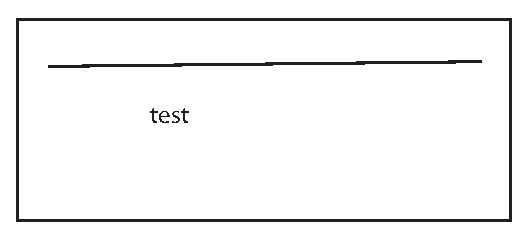
\includegraphics{testgraphic.eps}
\caption{A Test Graphic}
\end{figure}

\end{document}
